\section{Auswertung}
\label{sec:Auswertung}

\subsection{Spektrum eines $\ce{^{137}Cs}$-Strahlers}

  \noindent Es wird das Spektrum des im Versuchs benutzten Strahlers mithilfe des $\ce{NaI}$-Szintillationsdetektors aufgezeichnet. 
  In der \autoref{fig:spektrum} ist die Anzahl der Ereignisse in einem bestimmten Channel histogrammiert. 

  \begin{figure}[H]
    \centering
    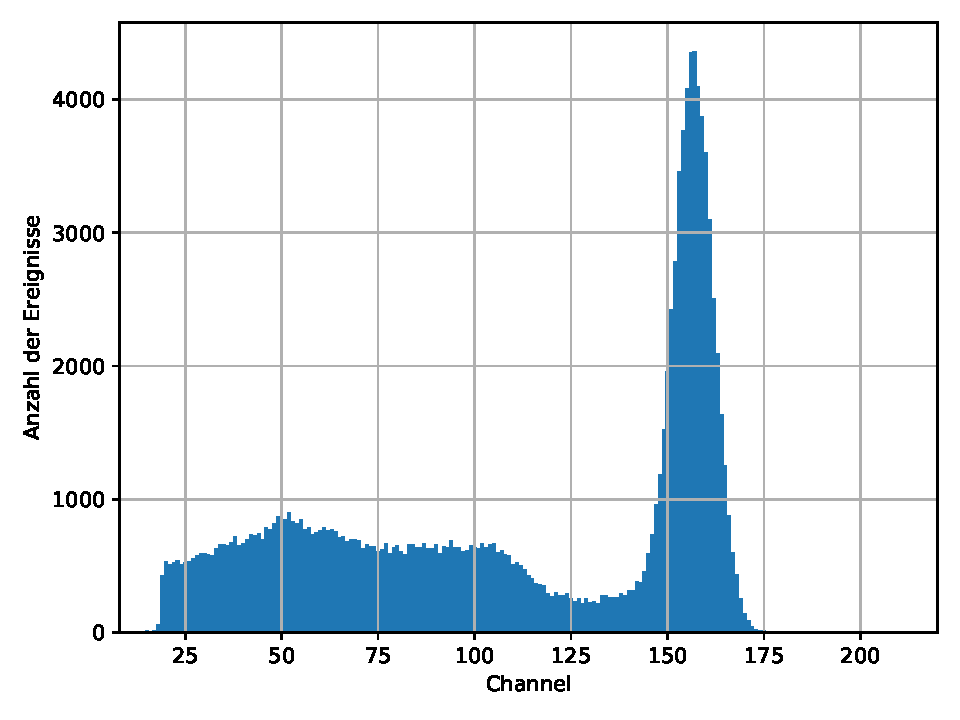
\includegraphics[width=\textwidth]{build/spektrum.pdf}
    \caption{Das Spektrum der $\ce^{137}Cs$-Quelle, aufgenommen mit einem $\ce{NaI}$-Szintillationsdetektor.}
    \label{fig:spektrum}
  \end{figure}

  \noindent In der \autoref{fig:spektrum} ist bei ungefähr Channel 50 der Rückstrahlpeak zu sehen und bei ungefähr Channel 105 die Comptonkante. 
  Der Photopeak befindet sich ungefähr bei Channel 165, dies entspricht einer Energie von ....


\subsection{Würfel 1}

  \noindent Zuerst wird ein leerer Würfel gemessen, welcher nur aus der Aluminiumhülle besteht, die alle folgenden Würfel umgibt. Diese Zählraten $R_0$ werden
  dementsprechend in den nachfolgenden Rechnungen als Nullmessung genutzt. \\
  Die aufgenommenen Werte, die Anzahl $N$ der Ereignisse, sind in der \autoref{tab:w1} zu finden mit der jeweiligen Zählrate $R_0$,  die Aufnahmezeit beträgt jeweils
   $t = \SI{300}{\second}$. Es wird nur der Channel mit der höchsten Anzahl an Ereignissen zur Auswertung genommen, da es sich hierbei um den Channel unter dem Photopeak handelt. 

  \begin{table}[H]
    \centering
    \caption{Die gemessene Anzahl der Ereignisse und die entsprechende Zählrate der Messung des leeren Würfel 1, der nur aus der Aluminiumhülle besteht.}
    \label{tab:w1}
    \begin{tabular}{c S[table-format=4.1] @{${}\pm{}$} S[table-format=2.1] S[table-format=2.2] @{${}\pm{}$} S[table-format=1.2]}
        \toprule
        {Strahlengang} & \multicolumn{2}{c}{$N$} & \multicolumn{2}{c}{$R_0 \mathbin{/} \left(\si{\per\second}\right)$} \\
        \midrule
        Hauptdiagonale ($I_2$) &  4148.0 & 64.4  &  13.83 & 0.22  \\ 
        Nebendiagonale ($I_1$) &  4098.0 & 64.0  &  13.66 & 0.21  \\ 
        Gerade ($I_5$)         &  4038.0 & 63.5  &  13.46 & 0.21  \\ 
        \bottomrule 
    \end{tabular}
  \end{table}

  \noindent Der Fehler der Anzahl der Ereignisse bestimmt sich als Poissonverteilt und beträgt somit $\sigma_N =\sqrt{N}$. Nach dem Zusammenhang 
  \begin{equation*}
    R = \frac{N}{t}
  \end{equation*}
  und der Gauß'schen Fehlerfortpflanzung ergibt sich der Fehler der Zählraten zu
  \begin{equation*}
    \sigma_R = \sqrt{\sigma_N^2 \left(\frac{1}{t}\right)^2 + \sigma_t \left(- \frac{N}{t^2}\right) } = \frac{\sigma_N}{t} \, ,
  \end{equation*}
  wobei im letzten Schritt $\sigma_t = 0 $ gesetzt wird. 
  
\subsection{Würfel 2}

  \noindent Der Würfel 2 ist homogen, daher werden nicht alle 12 Projektionen gemessen. Die maximale Anzahl der Ereignisse in einem Channel sind mit 
  Fehler in der \autoref{tab:w2} zu finden neben der jeweiligen Zählrate. Die Messzeit beträgt auch hier immer $t = \SI{300}{\second}$. Der 
  Absorptionskoeffizient berechnet sich dann nach 
  \begin{equation*}
    \mu = \frac{\ln\left(\frac{R_0}{R}\right)}{d} \, ,
  \end{equation*}
  wobei $R_0$ die Nullmessung der entsprechenden Projektion ist und $d$ die Stecke, welche die Gamma-Strahlung durch die Würfelebene zurücklegt. 
  
  \begin{table}[H]
    \centering
    \caption{Die Messwerte und daraus errechneten Werte der Messung des Würfel 2.}
    \label{tab:w2}
    \begin{tabular}{c S[table-format=4.1] @{${}\pm{}$} S[table-format=2.1] S[table-format=3.2] @{${}\pm{}$} S[table-format=1.2] S[table-format=1.6] @{${}\pm{}$} S[table-format=1.6]}
      \toprule
      {Projektion} & \multicolumn{2}{c}{$N$} & \multicolumn{2}{c}{$R \mathbin{/} \left(\si{\per\second}\right)$} & \multicolumn{2}{c}{$\mu \mathbin{/} \left(\si{\per\centi\metre}\right)$} \\
      \midrule
      $I_1$ & 2567.0 & 50.7 &  8.56 & 0.17 & 0.165379 & 0.008899 \\
      $I_2$ & 2213.0 & 47.0 &  7.38 & 0.16 & 0.148086 & 0.006205 \\
      $I_7$ & 3035.0 & 55.1 & 10.12 & 0.18 & 0.106168 & 0.008467 \\
      $I_8$ & 3159.0 & 56.2 & 10.53 & 0.19 & 0.064198 & 0.005566 \\
      $I_{11}$& 3298.0 & 57.4 & 10.99 & 0.19 & 0.067478 & 0.007823 \\
      $I_{12}$& 3187.0 & 56.5 & 10.62 & 0.19 & 0.078890 & 0.007898 \\
      \bottomrule  
    \end{tabular}
  \end{table}

  \noindent Für den Absorptionskoeffizienten des Materials, aus dem der Würfel 2 besteht, wird über die Werte in \autoref{tab:w2} gemittelt und es 
  ergibt sich der Wert:
  \begin{equation*}
    \mu_{\text{Würfel 2}} = \SI{0.105033(6547)}{\per\centi\metre} 
  \end{equation*}

\subsection{Würfel 3}

  \noindent Der Würfel 3 ist, genauso wie der Würfel 2, homogen, sodass wieder nicht alle Projektionen gemessen werden. Die aufgenommenen Werte sind 
  in der \autoref{tab:w3} zu finden, die Berechnung erfolgt analog der Rechnung zu Würfel 2. Die Messzeit beträgt hier $t= \SI{600}{\second}$. 

  \begin{table}[H]
    \centering
    \caption{Die Messwerte und daraus errechneten Werte der Messung des Würfel 3.}
    \label{tab:w3}
    \begin{tabular}{c S[table-format=3.1] @{${}\pm{}$} S[table-format=2.1] S[table-format=2.2] @{${}\pm{}$} S[table-format=1.2] S[table-format=1.6] @{${}\pm{}$} S[table-format=1.6]}
      \toprule
      {Projektion} & \multicolumn{2}{c}{$N$} & \multicolumn{2}{c}{$R \mathbin{/} \left(\si{\per\second}\right)$} & \multicolumn{2}{c}{$\mu \mathbin{/} \left(\si{\per\centi\metre}\right)$} \\
      \midrule
      $I_5$& 202.0 & 14.2 & 0.34 & 0.02 & 1.229461 & 0.024033 \\
      $I_7$& 203.0 & 14.2 & 0.34 & 0.02 & 1.307510 & 0.025422 \\
      $I_8$& 184.0 & 13.6 & 0.31 & 0.02 & 0.897694 & 0.017757 \\
      \bottomrule  
    \end{tabular}
  \end{table}

  \noindent Der gemittelte Wert des Absorptionskoeffizienten ergibt sich dann zu:
  \begin{equation*}
    \mu_{\text{Würfel 3}} = \SI{1.144888(59224)}{\per\centi\meter}
  \end{equation*}

\subsection{Würfel 4}

  \noindent Der Würfel 4 besteht aus 27 kleineren Würfel unterschiedlicher Materialien. Es wird eine Ebene des Würfels aus 9 kleineren Würfeln mit 
  allen 12 Projektionen ausgemessen. Damit ist das Gleichungssystem überbestimmt, sodass ein Least-Squares Fit durchgeführt wird. Für die 
  Absorptionskoeffizienten gilt die Gleichung \eqref{eqn:matrix} und es ergibt sich folgender Lösungsansatz:
  \begin{equation*}
    \vec{\mu} = \left( A^\top \cdot A \right)^{-1} \cdot A^\top \vec{I}
  \end{equation*}
  Die Fehler der $\mu_i$ stehen quadriert auf der Hauptdiagonale der Kovarianzmatrix $V[\vec{\mu}]$, welche sich wie folgt berechnet:
  \begin{equation*}
    V[\vec{\mu}] = \left( A^\top \cdot A \right)^{-1} \cdot A^\top V[\vec{I}] A \cdot \left( \left(A^\top \cdot A\right)^{-1} \right)^\top
  \end{equation*}
  Die Kovarianzmatrix $V[\vec{I}]$ ist eine Diagonalmatrix mit den Varianzen der $\vec{I}_i$ auf der Hauptdiagonale, da diese nicht korreliert sind.\\ 
  In der \autoref{tab:w4} sind die größten Anzahlen an Ereignissen aus einem Channel neben der daraus errechneten Zählraten.
  % Außerdem sind dort die Gesamtanzahl 
  % an Ereignissen pro Messung und die daraus errechneten Zählraten eingetragen. Es werden die Absorptionskoeffizienten aus beiden Werten gerechnet. 
  Die Messzeit beträgt $t =  \SI{300}{\second}$. 

  \begin{table}[H]
    \centering
    \caption{Die gemessenen Anzahlen der Ereignisse unter dem Photopeak und die daraus errechneten Werte $I_i$ von der Messung des Würfel 4.}
    \label{tab:w4}
    \begin{tabular}{c S[table-format=4.1] @{${}\pm{}$} S[table-format=2.1] S[table-format=1.2] @{${}\pm{}$} S[table-format=1.2] }
      \toprule
      {Projektion} & \multicolumn{2}{c}{$N$} & \multicolumn{2}{c}{$I \mathbin{/} \left(\si{\per\second}\right)$} \\
      \midrule
      $I_1 $   &  849.0 & 29.1 &  1.57 & 0.04 \\
      $I_2 $   &  482.0 & 22.0 &  2.15 & 0.05 \\
      $I_3 $   &  946.0 & 30.8 &  1.47 & 0.04 \\
      $I_4 $   &  655.0 & 25.6 &  1.82 & 0.04 \\
      $I_5 $   &  910.0 & 30.2 &  1.49 & 0.04 \\
      $I_6 $   & 1031.0 & 32.1 &  1.37 & 0.03 \\
      $I_7 $   &  618.0 & 24.9 &  1.89 & 0.04 \\
      $I_8 $   &  550.0 & 23.5 &  2.02 & 0.05 \\
      $I_9 $   &  706.0 & 26.6 &  1.76 & 0.04 \\
      $I_{10}$ & 3064.0 & 55.4 &  0.28 & 0.02 \\
      $I_{11}$ &  158.0 & 12.6 &  3.24 & 0.08 \\
      $I_{12}$ & 3041.0 & 55.1 &  0.28 & 0.02 \\
      \bottomrule
    \end{tabular}
  \end{table}

  % \begin{table}[H]
    % \centering
    % \caption{Die gemessenen Anzahlen der Ereignisse unter dem Photopeak und die daraus errechneten Werte $I_i$ von der Messung des Würfel 4.}
    % \label{tab:w4}
    % \begin{tabular}{c S[table-format=4.1] @{${}\pm{}$} S[table-format=2.1] S[table-format=1.2] @{${}\pm{}$} S[table-format=1.2] S[table-format=6.1] @{${}\pm{}$} S[table-format=3.1] S[table-format=1.2] @{${}\pm{}$} S[table-format=1.2]}
      % \toprule
      % & multicolumn{4}{c}{Channel unterm Photopeak} & \multicolumn{4}{c}{Gesamtanzahl}\\
      % \cmidrule(lr){2-5} \cmidrule(lr){6-9} 
      % {Projektion} & \multicolumn{2}{c}{$N$} & \multicolumn{2}{c}{$I \mathbin{/} \left(\si{\per\second}\right)$} & \multicolumn{2}{c}{$N$} & \multicolumn{2}{c}{$I \mathbin{/} \left(\si{\per\second}\right)$} \\
      % \midrule
      % $I_1 $   &  849.0 & 29.1 &  1.57 & 0.04 &  34201.0  & 184.9 & 1.28 & 0.01 \\
      % $I_2 $   &  482.0 & 22.0 &  2.15 & 0.05 &  21227.0  & 145.7 & 1.76 & 0.01 \\
      % $I_3 $   &  946.0 & 30.8 &  1.47 & 0.04 &  30051.0  & 173.4 & 1.41 & 0.01 \\
      % $I_4 $   &  655.0 & 25.6 &  1.82 & 0.04 &  37874.0  & 194.6 & 1.19 & 0.01 \\
      % $I_5 $   &  910.0 & 30.2 &  1.49 & 0.04 &  34459.0  & 185.6 & 1.28 & 0.01 \\
      % $I_6 $   & 1031.0 & 32.1 &  1.37 & 0.03 &  35475.0  & 188.3 & 1.25 & 0.01 \\
      % $I_7 $   &  618.0 & 24.9 &  1.89 & 0.04 &  28057.0  & 167.5 & 1.48 & 0.01 \\
      % $I_8 $   &  550.0 & 23.5 &  2.02 & 0.05 &  23221.0  & 152.4 & 1.67 & 0.01 \\
      % $I_9 $   &  706.0 & 26.6 &  1.76 & 0.04 &  29713.0  & 172.4 & 1.42 & 0.01 \\
      % $I_{10}$ & 3064.0 & 55.4 &  0.28 & 0.02 & 100770.0  & 317.4 & 0.21 & 0.00 \\
      % $I_{11}$ &  158.0 & 12.6 &  3.24 & 0.08 &   9760.0  &  98.8 & 2.54 & 0.01 \\
      % $I_{12}$ & 3041.0 & 55.1 &  0.28 & 0.02 &  90083.0  & 300.1 & 0.32 & 0.00 \\
      % \bottomrule
    % \end{tabular}
  % \end{table}

  \noindent Die mithilfe des Least-Squares-Fittes bestimmten Absorptionskoeffizienten $\vec{\mu}_i$ sind in der \autoref{tab:mu4} zu finden. 
  Dabei stehen die Absorptionskoeffizienten der Stoffe, die am nächsten an den ermittelten Werte liegen. 
  % Für die Identifizierung werden nur die Ergebnisse 
  % benutzt, bei denen die Anzahl der Ereignisse unter des Photopeaks benutzt werden. Die andere Berechnung steht zum Vergleich noch daneben. 

  \begin{table}[H]
    \centering
    \caption{Die ermittelten Werte für die Absorptionskoeffizienten der verschiedenen kleineren Würfel neben dem vermuteten Stoff.}
    \label{tab:mu4}
    \begin{tabular}{c S[table-format=1.6] @{${}\pm{}$} S[table-format=1.6] S[table-format=1.6] c}
      \toprule
      {Würfel} & \multicolumn{2}{c}{$\mu \mathbin{/} \left(\si{\per\centi\metre}\right)$} & {$\mu_{\text{lit}} \mathbin{/} \si{\per\centi\metre}$} & {Stoff} \\
      \midrule
      1 & 0.238148 & 0.024145 & 0.211 & Aluminium \\
      2 & 1.148348 & 0.023789 & 1.415 & Blei \\
      3 & 0.276631 & 0.024831 & 0.211 & Aluminium \\
      4 & 0.080247 & 0.020428 & 0.121 & Delrin \\
      5 & 1.154867 & 0.025784 & 1.415 & Blei \\
      6 & 0.089066 & 0.020524 & 0.121 & Delrin \\
      7 & 0.100641 & 0.023762 & 0.121 & Delrin \\
      8 & 1.063031 & 0.023457 & 1.415 & Blei \\
      9 & 0.045804 & 0.023045 & 0.121 & Delrin \\
      \bottomrule
    \end{tabular}
  \end{table}

  % \begin{table}[H]
    % \centering
    % \caption{Die ermittelten Werte für die Absorptionskoeffizienten der verschiedenen kleineren Würfel neben dem vermuteten Stoff.}
    % \label{tab:mu4}
    % \begin{tabular}{c S[table-format=1.6] @{${}\pm{}$} S[table-format=1.6] S[table-format=1.6] @{${}\pm{}$} S[table-format=1.6] S[table-format=1.6] c}
      % \toprule
      % & \multicolumn{2}{c}{Channel unterm Photopeak} & \multicolumn{2}{c}{Gesamtanzahl} \\
      % \cmidrule(lr){2-3} \cmidrule(lr){4-5}
      % {Würfel} & \multicolumn{2}{c}{$\mu \mathbin{/} \left(\si{\per\centi\metre}\right)$} & \multicolumn{2}{c}{$\mu \mathbin{/} \left(\si{\per\centi\metre}\right)$} & {$\mu_{\text{lit}} \mathbin{/} \si{\per\centi\metre}$} & {Stoff} \\
      % \midrule
      % 1 & 0.238148 & 0.024145 & 0.147409 & 0.003774 & 0.211 & Aluminium \\
      % 2 & 1.148348 & 0.023789 & 0.847626 & 0.003467 & 1.415 & Blei \\
      % 3 & 0.276631 & 0.024831 & 0.090092 & 0.003808 & 0.211 & Aluminium \\
      % 4 & 0.080247 & 0.020428 & 0.088445 & 0.003151 & 0.121 & Delrin \\
      % 5 & 1.154867 & 0.025784 & 0.944886 & 0.003727 & 1.415 & Blei \\
      % 6 & 0.089066 & 0.020524 & 0.154456 & 0.003197 & 0.121 & Delrin \\
      % 7 & 0.100641 & 0.023762 & 0.199140 & 0.003842 & 0.121 & Delrin \\
      % 8 & 1.063031 & 0.023457 & 0.873086 & 0.003481 & 1.415 & Blei \\
      % 9 & 0.045804 & 0.023045 & 0.078337 & 0.003784 & 0.121 & Delrin \\
      % \bottomrule
    % \end{tabular}
  % \end{table}